\section{Неспециализированные вычисления на графических процессорах}

Прообразом первых графических процессоров, появившихся в 90-е~годы
\rom{20}~века, были специализированные чипы аркадных автоматов. Их использование было обусловлено малыми объёмами оперативной памяти, что не позволяло хранить в ней кадры перед отправкой на устройство видеовывода. В
дальнейшем разделение вычислений на графические и неграфические лишь
усугубилось, что оказало существенное влияние на архитектуру современных
компьютеров.

В начале \rom{21}~века графические процессоры получили поддержку шейдеров и возможность работы с числами с плавающей запятой. Это событие положило начало ряду экспериментов с организацией неграфических параллельных
расчётов на графических процессорах. При помощи графических API данные
передавались в виде текстур, а расчётные программы --- в виде шейдеров~\cite{Berillo}.
Таким образом учёные начали производить вычисления, связанные с матрицами и векторами, на ГПУ. Первой программой, выполнившейся заметно быстрее
на ГПУ, чем на ЦПУ, стала реализация LU-разложения, описанная в работе~\cite{Galoppo}.

С увеличением популярности использования ГПУ для научных расчётов
начали формироваться идеи фреймворков общего назначения, позволяющих
отойти от графической парадигмы работы с данными и отказаться от использования OpenGL или DirectX. Такими фреймворками впоследствии стали технологии NVIDIA CUDA и OpenCL.

\subsection{Краткий обзор технологии NVIDIA CUDA}

Первоначальная версия NVIDIA CUDA SDK была представлена 15~февраля~2007~г.
В основе NVIDIA CUDA API лежит диалект языка C++.

Для компиляции программ NVIDIA CUDA SDK предлагает специализированный компилятор nvcc. При этом код программ разделяется на host-часть, выполняющуюся ЦПУ, и device-часть, выполняющуюся графическим процессором. В результате получаются как минимум два объектных файла, готовых к сборке в
конечный исполняемый файл в любой среде программирования~\cite{CUDADoc}.

По сравнению с использовавшимся ранее подходом к организации вычислений общего назначения посредством возможностей графических API, архитектура CUDA имеет ряд преимуществ:
\begin{itemize}
\item использование диалекта языка C++, что позволяет упростить процесс изучения архитектуры;
\item  полная аппаратная поддержка целочисленных и побитовых операций;
\item  разделяемая между потоками память размером в 16 Кбайт может быть
использована под организованный пользователем кэш с более широкой полосой пропускания, чем при выборке из обычных текстур.
\end{itemize}

\subsection{Краткий обзор технологии OpenCL}

OpenCL --- фреймворк для написания компьютерных программ, реализующих
параллельные вычисления на различных графических и центральных
процессорах, а также ППВМ. В OpenCL входят язык программирования, базирующийся на стандарте C99, и интерфейс программирования приложений.

Основной задачей проекта OpenCL является создание и поддержка открытого стандарта, позволяющего разрабатывать универсальные программы для параллельных вычислений на различных процессорах и создавать вычислительные машины,
использующие несколько процессоров различных архитектур одновременно.

OpenCL рассматривает компьютерную систему как совокупность вычислительных устройств (ЦПУ и ГПУ), подключённых к управляющему ЦПУ, называемому хостом. Функции, предназначенные для выполнения на вычислительных устройствах, называются функциями-ядрами и могут выполняться параллельно на нескольких устройствах.

\subsection{Иерархия потоков выполнения в NVIDIA CUDA}

Как упоминалось ранее, одной из особенностей написания программ с использованием технологии NVIDIA CUDA является разделение всего программного кода
на host- и device-части. Для этого используются спецификаторы функций:
\begin{itemize}
\item \texttt{\_\_host\_\_} --- код предназначен для выполнения на ЦПУ (используется по умолчанию );
\item \texttt{\_\_device\_\_} --- код предназначен для выполнения на вычислительном устройстве;
\item \texttt{\_\_global\_\_} --- особый спецификатор для так называемых функций-ядер (kernel), которые запускаются с центрального процессора, а работают на видеокарте.
\end{itemize}

Остановимся подробнее на \textit{функциях-ядрах}. Их отличие от обычных
функций языка C++ заключается в том, что при вызове они выполняются N раз
параллельно в N потоках выполнения. При этом количество потоков выполнения, которые можно создать на ГПУ, практически не ограничено.

Для организации работы со столь большим количеством потоков используется иерархическая структура: потоки объединяются в варпы (warp), варпы, в
свою очередь, --- в блоки (block), а блоки составляют сетку (grid).

\textit{Варп} --- это минимальная независимая от других единица выполнения кода. Размер варпа всегда равен 32 потокам. Эти потоки всегда выполняются физически синхронно. \textit{Блок} --- это автономная группа потоков. Взаимодействия
потоков между блоками невозможны.

% TODO: Center the code

Вызов функции-ядра осуществляется следующим образом:

\texttt{kernel\_name<{<}<grid\_size, block\_size>{>}>(arguments);}

В тройных угловых скобках в участке программного кода выше указываются размеры сетки и блока.

Примером может послужить программа для перемножения матриц: она
иллюстрирует параллельное выполнения потоков с помощью многократного
повторения операции сложения с разными числами.

\begin{lstlisting}
__global__ void MatAdd(
	float A[N][N], float B[N][N], float C[N][N])
{
	int i = threadIdx.x;
	int j = threadIdx.y;
	C[i][j] = A[i][j] + B[i][j];
}

int main()
{
	...
	int numBlocks = 1;
	dim3 threadsPerBlock(N, N);
	MatAdd<<<numBlocks, threadsPerBlock>>>(A, B, C);
	...
}
\end{lstlisting}

Во фрагменте исходного кода выше \texttt{threadIdx} --- трёхкомпонентный вектор, хранящий координаты потока в блоке (рис.~\ref{fig:ThreadsStructure}). Таким образом, видим: имеется один блок размеров N$ \times $N и три массива той же размерности. Каждому потоку ставится в соответствие по одному элементу каждой из трёх матриц. Следовательно, все потоки покрывают все элементы матриц. 

% Рисунок 2.1
\afterpage{\clearpage}\begin{figure}[p]
\centering
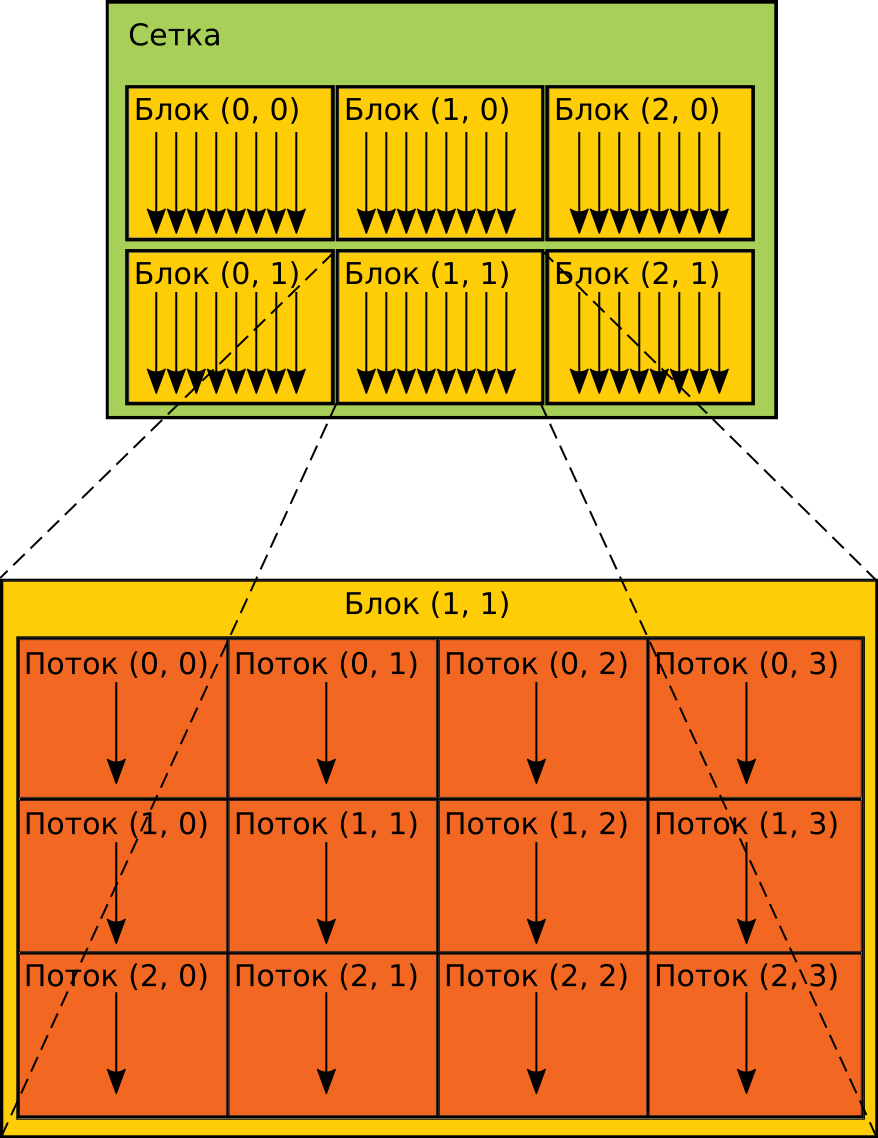
\includegraphics[width=0.5\textwidth]{include/graphics/image2}
\caption{Иерархическая структура потоков выполнения}
\label{fig:ThreadsStructure}
\end{figure}

\subsection{Иерархия памяти в NVIDIA CUDA}

Согласно статье~\cite{Frolov} в NVIDIA CUDA выделяют следующие виды памяти:
\begin{itemize}
\item регистры процессора --- блок ячеек памяти внутри процессора, из которой на каждый поток выполнения выделяются регистры;
\item локальная память --- участок глобальной памяти, обособленно выделяемой потоку при нехватке регистров;
\item глобальная память --- аналог оперативной памяти ПК и основной вид памяти, используемый для обмена данными между ЦПУ и ГПУ;
\item разделяемая память --- область памяти, одинаково адресуемой для всех потоков выполнения внутри блока;
\item константная память --- тип памяти, модификация которой возможна только с ЦПУ;
\item текстурная память --- интерфейс чтения глобальной памяти с использованием специфических для текстур операций.
\end{itemize}

Для каждого потока выделяется локальная память (регистровая и, опционально, дополнительная). Для каждого блока выделяется разделяемая память,
доступ к которой имеют все потоки блока. Разделяемая память выделена,
пока существует блок. Все существующие потоки имеют доступ к глобальной
памяти. Также каждый поток имеет доступ к чтению константной и текстурной
памяти. Глобальная, константная и текстурная память не перевыделяются на
протяжении работы программы, т. о. разные функции-ядра могут работать с
этими видами памяти (рис.~\ref{fig:MemoryStructure}).

\begin{figure}[p]
\centering
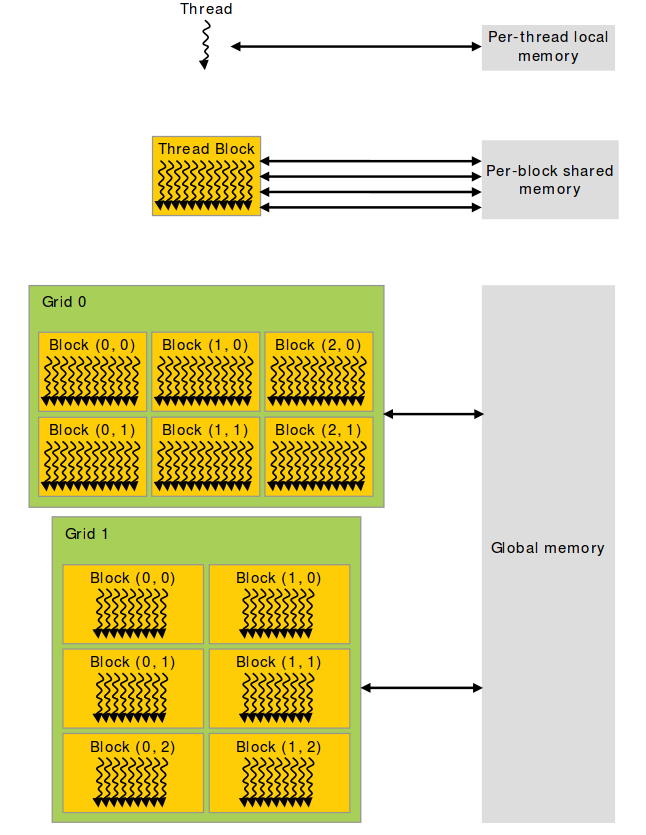
\includegraphics[width=1\textwidth]{include/graphics/image3}
\caption{Иерархическая структура памяти и права доступа к ней}
\label{fig:MemoryStructure}
\end{figure}

\subsection{Иерархия потоков выполнения в OpenCL}

Иерархическая модель потоков выполнения OpenCL концептуально не отличается от 
своего аналога от компании NVIDIA.

Аналогом потоков в OpenCL являются \emph{рабочие элементы} (\emph{work-item}). Они объединяются в \emph{рабочие группы} (\emph{work-group}), причём рабочие элементы, принадлежащие разным рабочим группам, не могут взаимодействовать.

На рис.~\ref{fig:WorkGroupsStructure} изображён пример \textit{двухмерного пространства индексов} (2D-range index space), являющегося аналогом сетки в NVIDIA CUDA. В общем случае пространство индексов является N-мерным.

\begin{figure}[p]
\centering
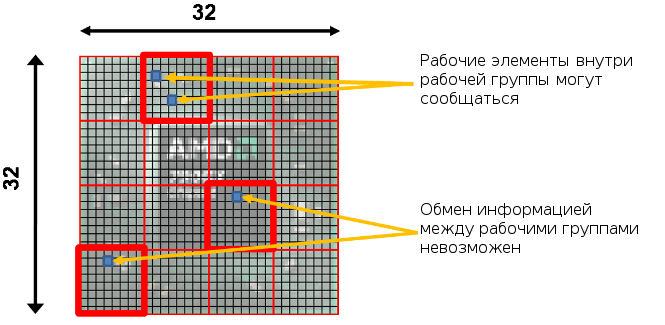
\includegraphics[width=1\textwidth]{include/graphics/image4}
\caption{Иерархическая структура рабочих групп}
\label{fig:WorkGroupsStructure}
\end{figure}

Данное пространство индексов разделено на 16 рабочих групп, имеющих
собственные координаты и размер 8$ \times $8. Рабочие элементы имеют два типа координат: локальные (относительно рабочей группы) и глобальные (относительно сетки целиком).

По аналогии с NVIDIA~CUDA используются функции-ядра, выполняющиеся на 
вычислительном устройстве.

\subsection{Иерархия памяти в OpenCL}

Так как хост и вычислительное устройство не имеют общего адресного
пространства, взаимодейстие между памятью хоста и памятью OpenCL-
устройства происходит посредством использования различных областей памяти (рис.~\ref{fig:OpenCLMemoryStructure}).

\begin{figure}[p]
\centering
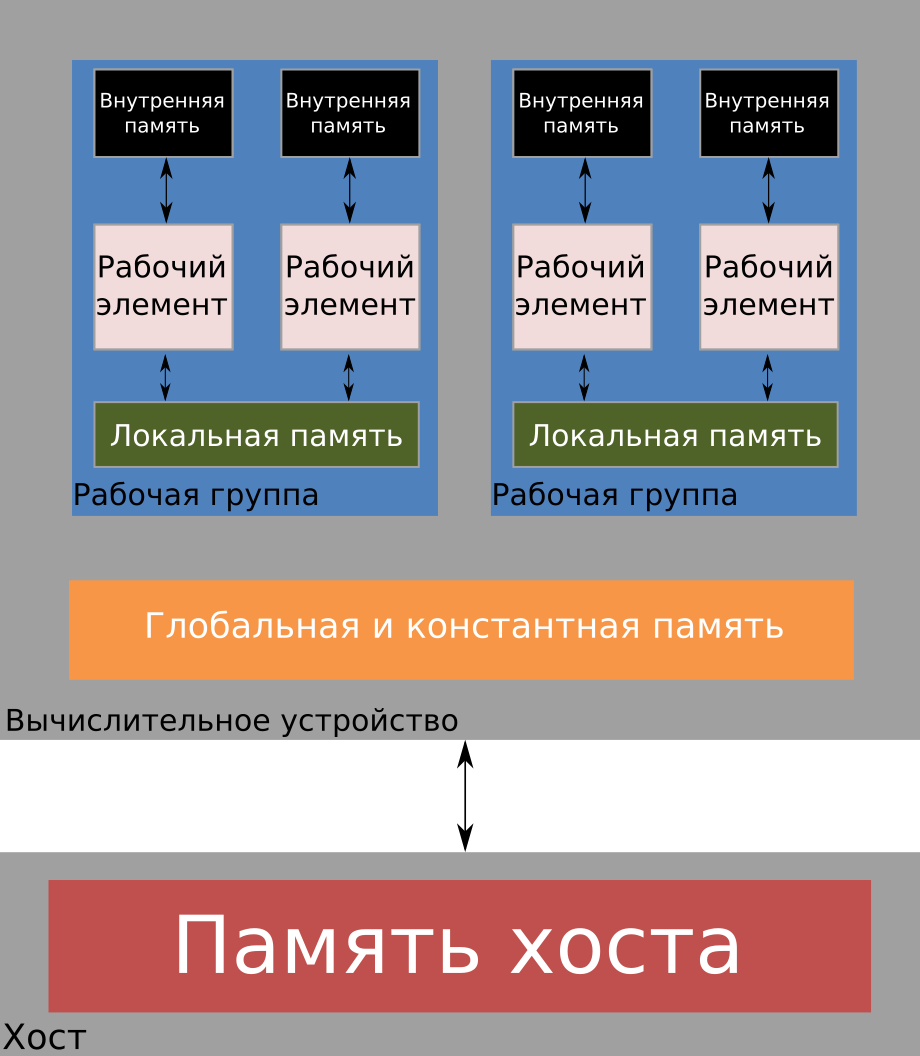
\includegraphics[width=0.5\textwidth]{include/graphics/image5}
\caption{Иерархия памяти в OpenCL}
\label{fig:OpenCLMemoryStructure}
\end{figure}

Глобальная память --- это участок памяти, к которому все рабочие элементы, группы, а также хост, имеют полный доступ (чтение и запись). Эта область
памяти может быть выделена только хостом.

Константная память --- это участок глобальной памяти, остающийся нетронутым на протяжении выполнения функции-ядра. Рабочие группы могут только читать данные из этой области, хост же имеет к ней полный доступ.

Локальная память --- это место обмена данными между рабочими элементами рабочей группы. Все элементы имеют полный доступ к этой области.

Внутренняя память --- это память, принадлежащая конкретному рабочему
элементу.

В большинстве случаев память хоста и память OpenCL-устройства работают независимо друг от друга. Соответственно, имеется специфика обмена данными между ними: необходимо перемещать данные из памяти хоста в глобальную память, затем в локальную, и обратно.

\subsection{Специфика работы с видеопамятью}

Перед организацией параллельных вычислений следует ознакомиться с некоторыми приёмами оптимизации, которые помогут сохранить производительность, выигранную от использования ГПУ. Наиболее широко распространённым и лёгким в освоении приёмом является согласованный доступ к памяти, аналогичный выравниванию памяти при работе ЦПУ с оперативной памятью.

Глобальная память физически расположена на device-устройстве, доступ к
которой происходит посредством 32-, 64- и 128-байтных транзакций. Необходимое условие для их существования --- обращение к выровненным участкам
памяти. Таковыми являются участки, адреса первых элементов которых кратны
32, 64 и 128 байтам соответственно.

Когда варп выполняет инструкцию, обращающуюся к глобальной памяти,
обращения каждого потока внутри варпа сливаются в одну или несколько транзакций, в зависимости от размера слова, запрашиваемого каждым потоком, и
разброса адресов, к которым обращаются потоки.

Команды работы с глобальной памятью поддерживают чтение и запись
слов размером 1, 2, 4, 8 и 16 байтов. Любой запрос к глобальной памяти возможен только в случае, если размер запрашиваемых данных равен 1, 2, 4, 8 или 16
байтам, и они выровнены (т.~е.~их адреса кратны размеру).

Затем одиночные запросы к глобальной памяти объединяются в транзакции. Например, запросы 32 потоков одного варпа, обращающиеся к четырём последовательно располагающимся байтам каждый, объединятся в транзакцию размером 128 байтов в том случае, если адрес, к которому обращается первый поток варпа, кратен 128 байтам.

\clearpage